
\chapter{Pengenalan Enterprise Architecture}

\section{Definisi 'Enterprise'}

\subsection{Oxford English Dictionary}
Menurut Oxford English Dictionary, 'Enterprise' didefinisikan sebagai sebuah proyek atau usaha yang biasanya membutuhkan upaya dan keberanian. Selain itu, juga merujuk pada inisiatif, yaitu keberanian untuk mengambil risiko demi mendapatkan keuntungan, serta dapat diartikan sebagai organisasi atau perusahaan bisnis.

\subsection{Cambridge English Dictionary}
Menurut Cambridge English Dictionary, 'Enterprise' merujuk pada kemampuan untuk memikirkan rencana baru dan membuatnya berhasil. Selain itu, istilah ini juga digunakan untuk menggambarkan sebuah perusahaan.

\subsection{Merriam-Webster Dictionary}
Menurut Merriam-Webster Dictionary, 'Enterprise' adalah proyek atau usaha yang sering kali memerlukan keberanian. Definisi ini juga mencakup kesiapan untuk terlibat dalam usaha yang berani dan penuh risiko, serta menggambarkan suatu unit ekonomi yang terorganisir.

\subsection{Kesimpulan Definisi 'Enterprise'}
Secara umum, 'Enterprise' mengacu pada proyek atau usaha yang berani dan penuh risiko. Selain itu, istilah ini juga dapat merujuk pada organisasi atau perusahaan bisnis. Definisi ini secara umum konsisten di antara kamus bahasa Inggris terkemuka.

\section{Definisi 'Arsitektur'}

\subsection{Oxford English Dictionary}
Menurut Oxford English Dictionary, 'Arsitektur' didefinisikan sebagai seni atau praktik merancang dan membangun bangunan. Istilah ini juga dapat merujuk pada gaya atau metode konstruksi serta tata letak atau struktur dari suatu benda.

\subsection{Cambridge English Dictionary}
Menurut Cambridge English Dictionary, 'Arsitektur' adalah seni dan praktik merancang bangunan. Selain itu, istilah ini juga digunakan untuk menggambarkan gaya atau desain dari bangunan tertentu atau sekelompok bangunan, serta cara sesuatu diatur atau disusun.

\subsection{Merriam-Webster Dictionary}
Menurut Merriam-Webster Dictionary, 'Arsitektur' adalah seni atau ilmu dalam merancang dan membangun bangunan. Definisi ini juga mencakup metode atau gaya konstruksi, serta bagaimana bagian-bagian dari suatu objek diatur atau disistematisasi.

\subsection{Ringkasan Definisi 'Arsitektur'}
Secara umum, 'Arsitektur' merujuk pada seni atau praktik merancang dan membangun bangunan. Selain itu, istilah ini juga dapat merujuk pada gaya atau metode konstruksi, serta cara bagian-bagian dari sesuatu diatur atau disistematisasi.

\section{Definisi 'Arsitektur' Menurut IEEE}
Menurut IEEE, 'Arsitektur' adalah organisasi mendasar dari suatu sistem, yang melibatkan komponen sistem dan hubungan antar komponen. Arsitektur juga mencakup manajemen desain dan evolusi sistem, di mana komponen sistem dapat berupa perangkat keras, perangkat lunak, data, orang, dan proses.

\section{Definisi 'Enterprise Architecture'}

\subsection{Menurut Gartner}
Menurut Gartner, 'Enterprise Architecture' adalah disiplin untuk perancangan, perencanaan, pelaksanaan, dan pengendalian proyek. Disiplin ini membantu organisasi mencapai konsistensi antara bisnis dan IT serta melibatkan kolaborasi antara berbagai pemangku kepentingan. 'Enterprise Architecture' juga dapat digunakan untuk membantu dalam pengambilan keputusan strategis.

\subsection{Menurut TOGAF}
Menurut TOGAF, 'Enterprise Architecture' adalah kerangka arsitektur yang memberikan definisi dan desain dasar untuk arsitektur perusahaan. Tujuan dari arsitektur ini adalah untuk memastikan agar operasi perusahaan berjalan secara konsisten dan efisien dengan fokus pada standar dan prosedur yang digunakan di dalam perusahaan.

\subsection{Menurut ISO/IEC/IEEE 42010}
Menurut ISO/IEC/IEEE 42010, 'Enterprise Architecture' adalah pendekatan mendasar terhadap organisasi suatu sistem. Pendekatan ini melibatkan pemahaman semua komponen, hubungan antara komponen, serta lingkungan tempat komponen tersebut beroperasi. Pendekatan ini menekankan pentingnya struktur dan interaksi dalam suatu sistem, serta menyediakan kerangka kerja untuk pemahaman dan desain sistem.

\section{Berbagai Kerangka Arsitektur Enterprise}
Berbagai kerangka arsitektur enterprise telah muncul seiring waktu untuk memandu organisasi dalam menyusun sistem TI dan bisnis mereka. Beberapa kerangka yang terkenal termasuk Business System Planning (BSP), PRISM Architecture Framework, NIST Enterprise Architecture Model, Zachman Framework, Enterprise Architecture Planning (EAP), Sherwood Applied Business Security Architecture (SABSA), dan Federal Enterprise Architecture Framework (FEAF). Kerangka-kerangka ini bertujuan untuk membantu organisasi dalam mengelola kompleksitas sistem mereka, memastikan keselarasan antara tujuan bisnis dan TI.

Kerangka arsitektur enterprise lainnya termasuk Gartner's Enterprise Architecture Method, Department of Defense Architecture Framework (DoDAF), Australian Government AGA, Business Architecture Body of Knowledge (BizBoK), dan ISO Standard for Enterprise Modeling (ISO19439).

\section{Business System Planning (BSP)}
Business System Planning (BSP) melibatkan pemahaman tujuan bisnis, menganalisis proses bisnis, dan merancang arsitektur sistem informasi yang mendukung proses tersebut. BSP membantu organisasi untuk meningkatkan efisiensi, menyederhanakan operasi, dan mengoptimalkan alokasi sumber daya.

\begin{center}
	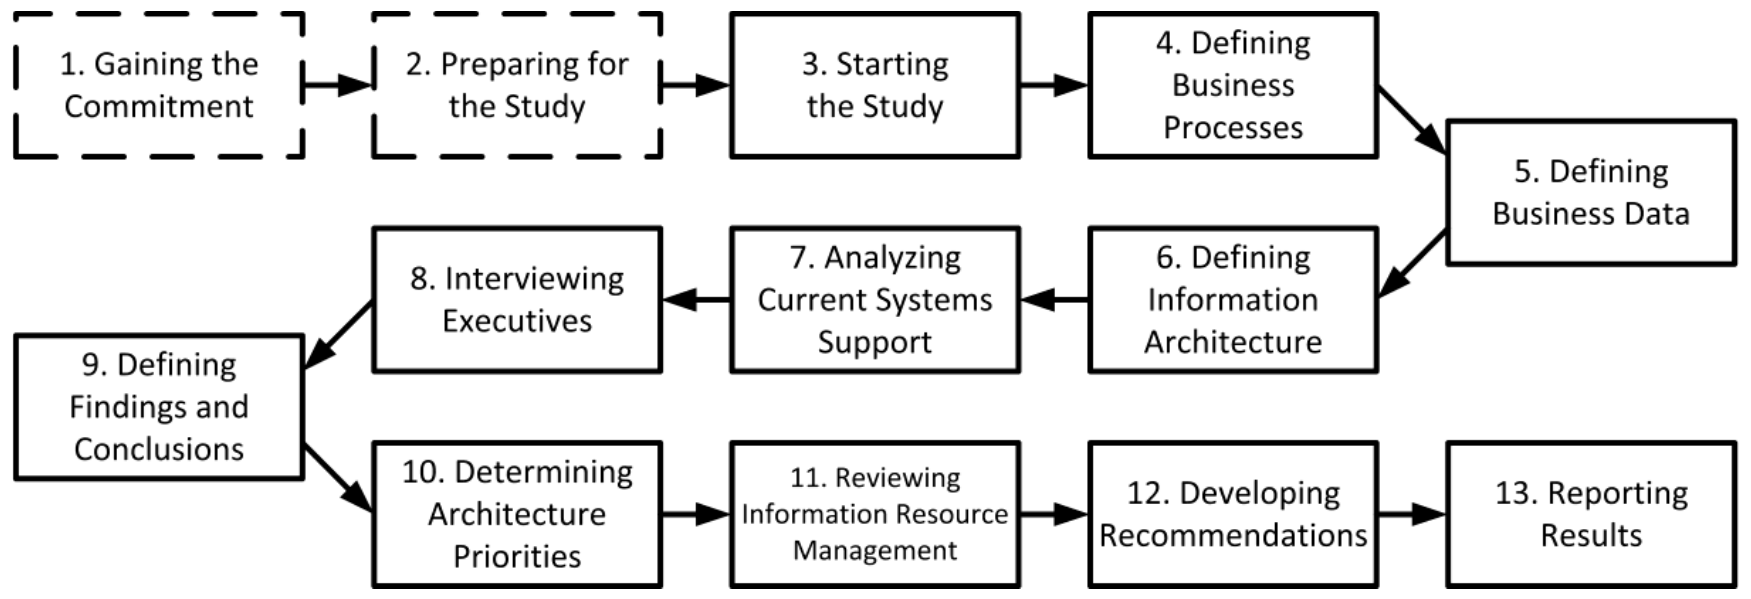
\includegraphics[width=\textwidth]{../figures/bsp}
\end{center}

\section{PRISM Architecture Framework}
PRISM Architecture Framework, atau Partnership for Research in Information Systems Management, merupakan salah satu kerangka arsitektur enterprise yang pertama kali dikembangkan oleh konsorsium vendor TI. Kerangka ini berfokus pada integrasi sistem dan teknologi informasi, membantu organisasi untuk memahami dan mengelola kompleksitas TI.

\begin{center}
	\begin{figure}[ht]
		\begin{minipage}[b]{0.49\linewidth}
			\centering
			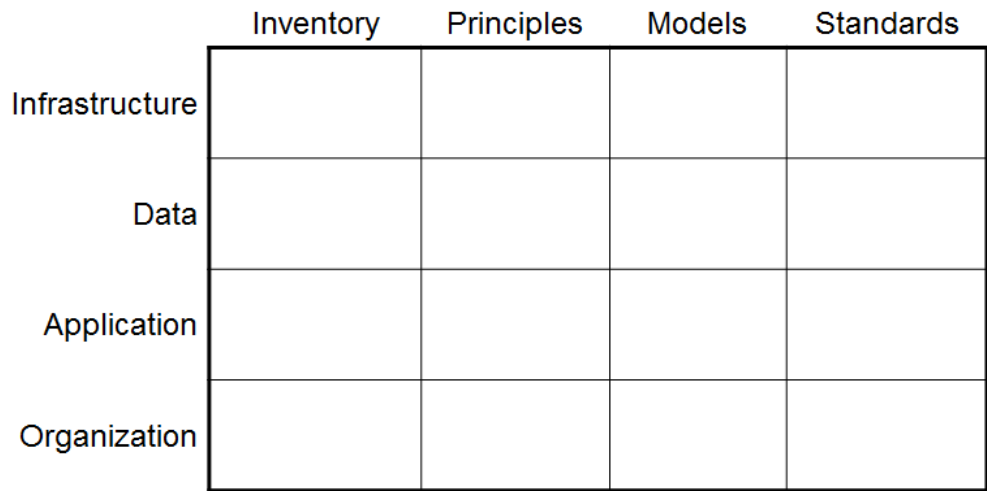
\includegraphics[width=\textwidth]{../figures/prism_matrix}
			\caption{matriks}
		\end{minipage}
		\hfill
		\begin{minipage}[b]{0.49\linewidth}
			\centering
			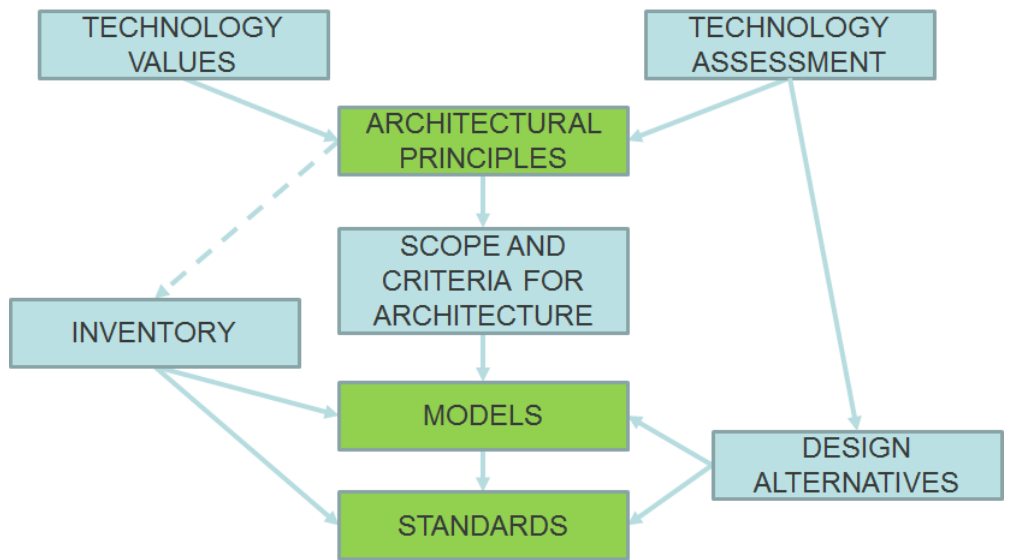
\includegraphics[width=\textwidth]{../figures/prism_relationships}
			\caption{hubungan}
		\end{minipage}
	\end{figure}
\end{center}

\section{NIST Enterprise Architecture Model}
Model Arsitektur Enterprise NIST, yang dikembangkan oleh National Institute of Standards and Technology, menekankan pada pengaturan dan organisasi operasi TI. Model ini membagi arsitektur TI menjadi lima tingkat yang meliputi bisnis, data, aplikasi, teknologi, dan hasil. Ini memungkinkan perencanaan strategis dan pengambilan keputusan berbasis data.

\begin{center}
	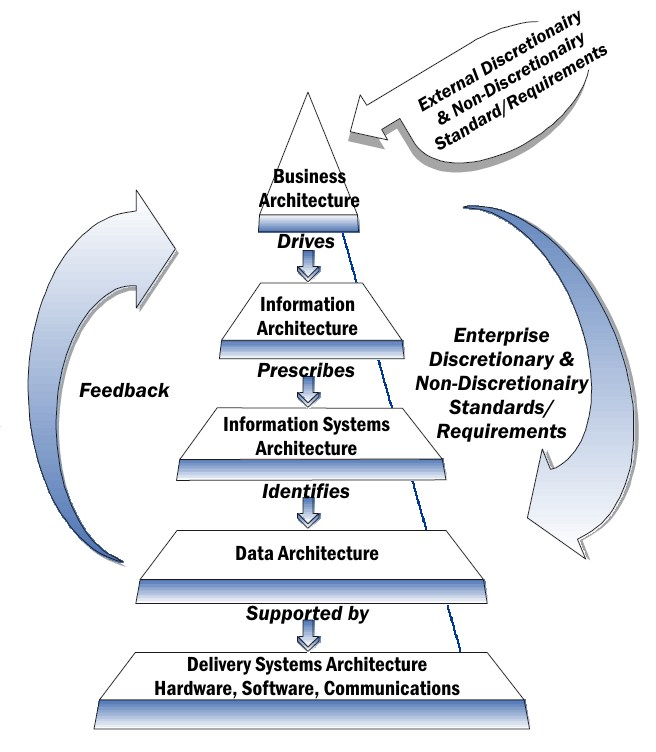
\includegraphics[width=.40\textwidth]{../figures/nist}
\end{center}

\section{Zachman Framework}
Zachman Framework adalah skema untuk memahami dan mengelola kompleksitas arsitektur enterprise, dibagi menjadi enam tingkat berbeda. Framework ini merangkum dari tingkat yang paling abstrak hingga yang paling konkret, cocok untuk berbagai jenis organisasi, dari bisnis hingga pemerintah.

\begin{center}
	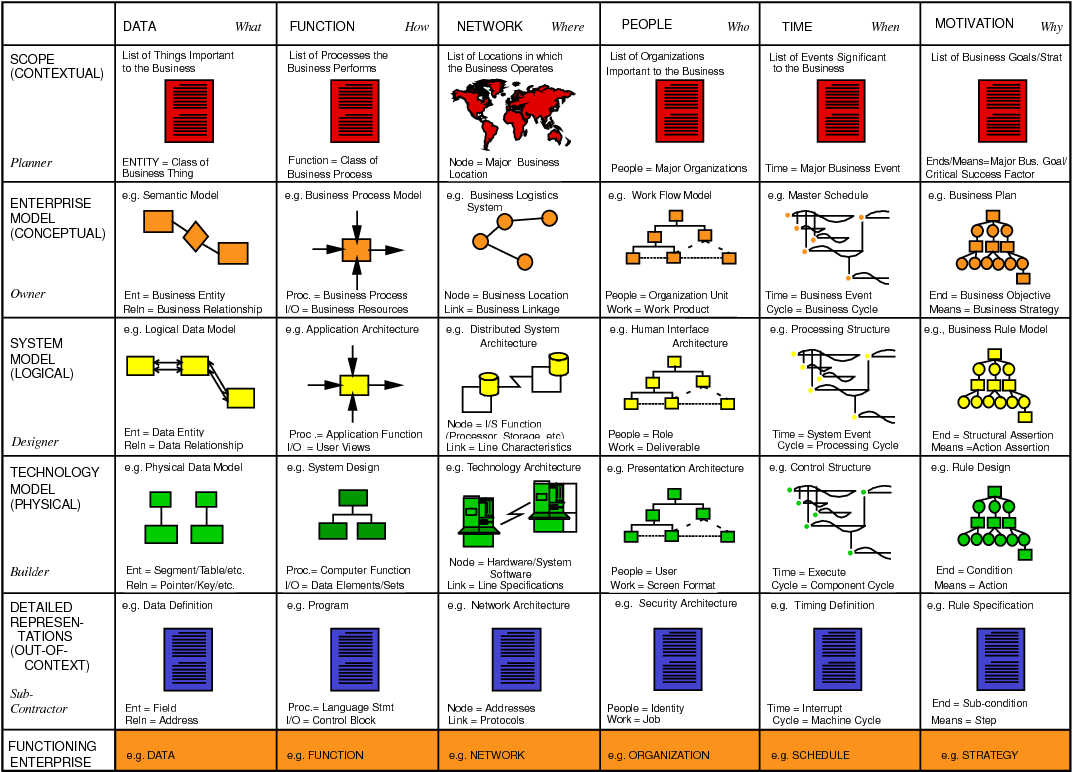
\includegraphics[width=0.76\textwidth]{../figures/zachman}
\end{center}

\section{Enterprise Architecture Planning (EAP)}
Enterprise Architecture Planning (EAP) mencakup metode perencanaan arsitektur sistem informasi. EAP bertujuan untuk mengidentifikasi kebutuhan bisnis dari teknologi informasi dan mengembangkan rencana untuk implementasi teknologi baru berdasarkan kebutuhan tersebut. Ini dapat membantu dalam transformasi digital dan perubahan organisasi.

\begin{center}
	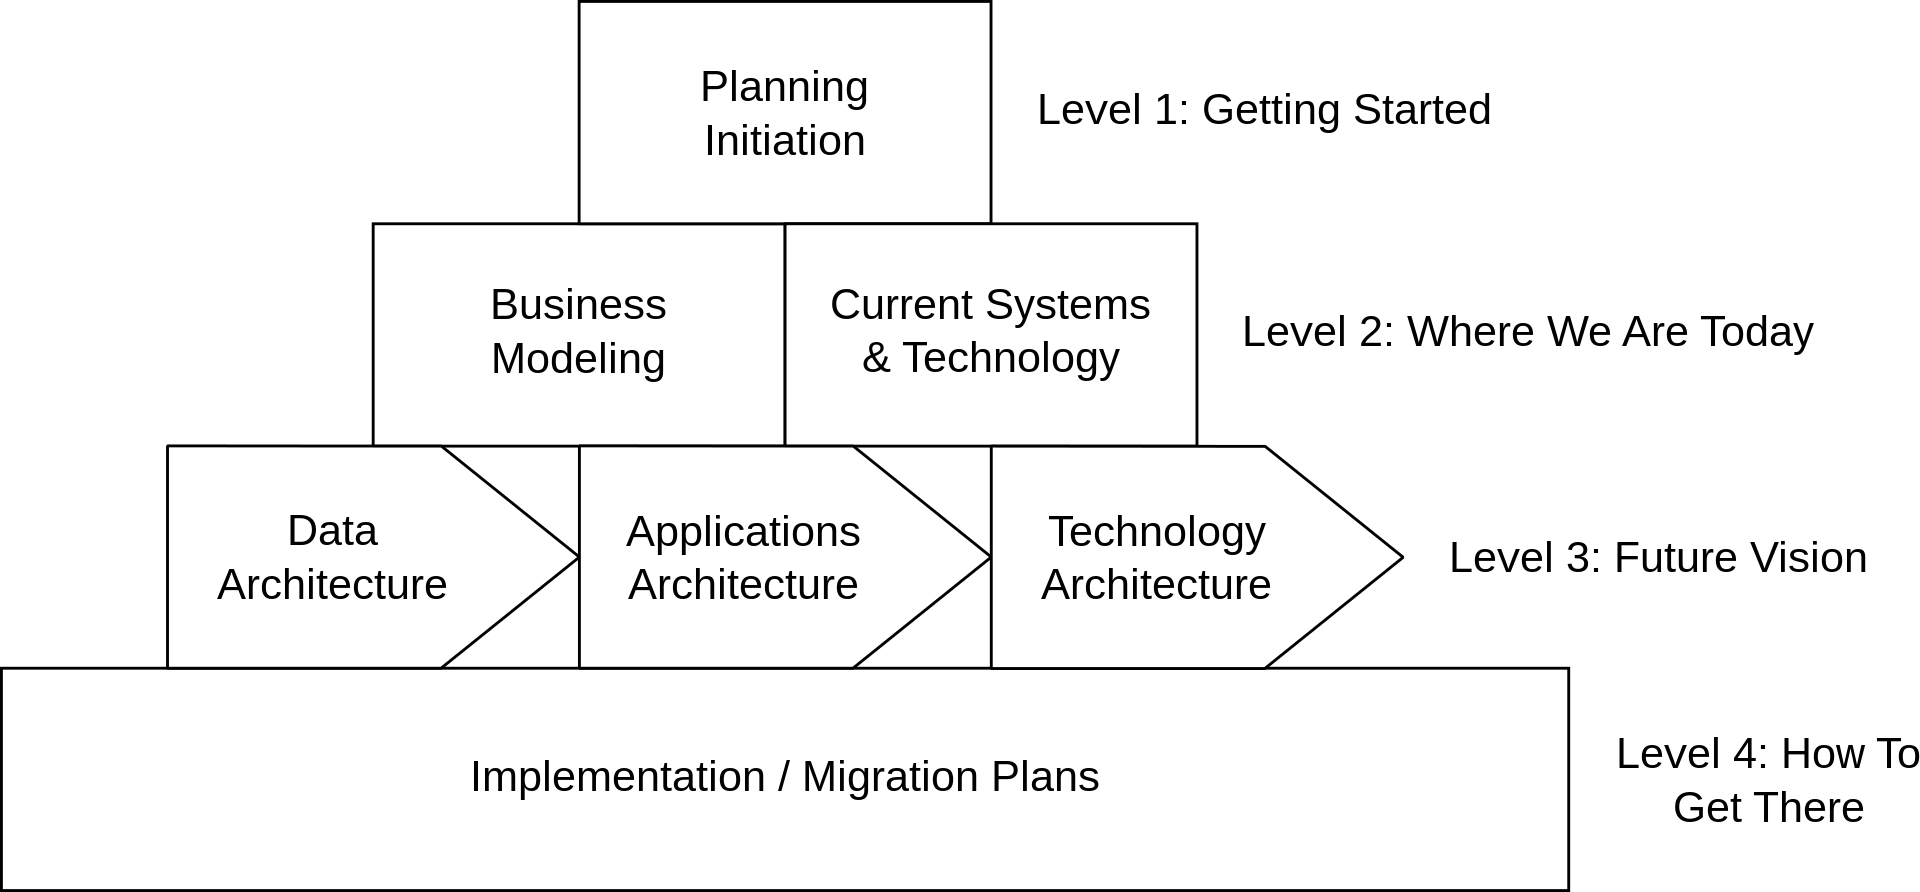
\includegraphics[width=1\textwidth]{../figures/eap}
\end{center}

\section{Sherwood Applied Business Security Architecture (SABSA)}
Sherwood Applied Business Security Architecture (SABSA) menyediakan model dan metodologi untuk mengembangkan kerangka kerja keamanan informasi dan manajemen risiko. SABSA dirancang dengan pendekatan "start-to-finish" dan "top-down" dan dapat disesuaikan dengan kebutuhan spesifik organisasi.

\begin{center}
	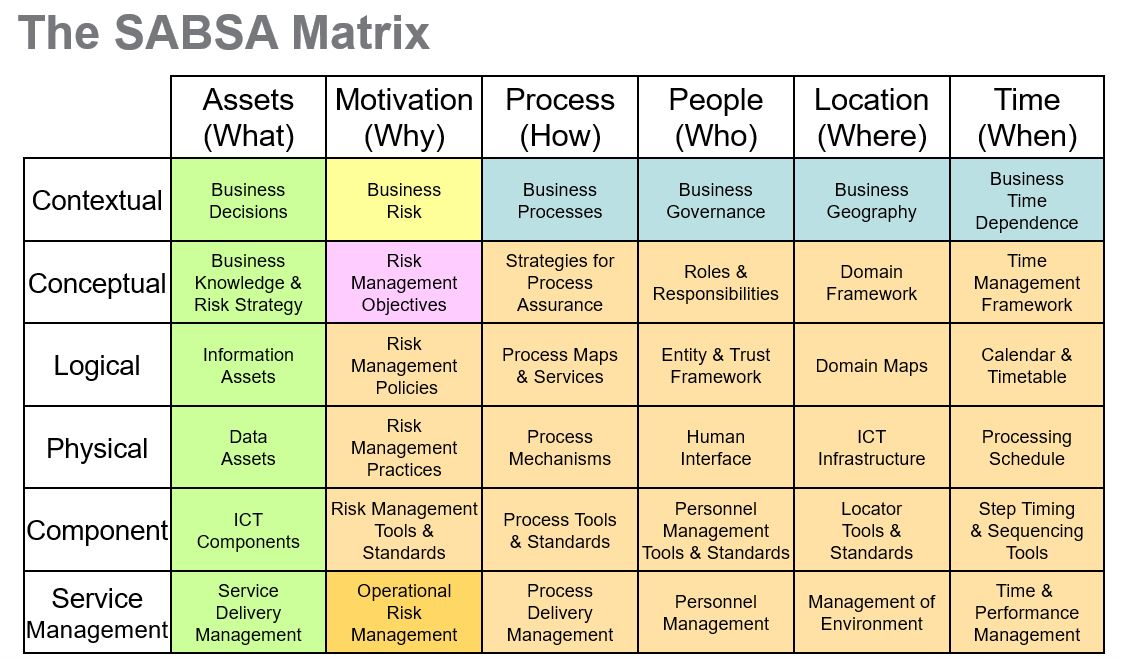
\includegraphics[width=0.8\textwidth]{../figures/sabsa}
\end{center}

\section{Federal Enterprise Architecture Framework (FEAF)}
Federal Enterprise Architecture Framework (FEAF) adalah kerangka kerja yang digunakan oleh pemerintah federal AS. FEAF membantu dalam meningkatkan efisiensi dan efektivitas layanan pemerintah, memfasilitasi kolaborasi antara agen dan departemen pemerintah, dan merupakan bagian dari strategi modernisasi TI pemerintah AS.

\begin{center}
	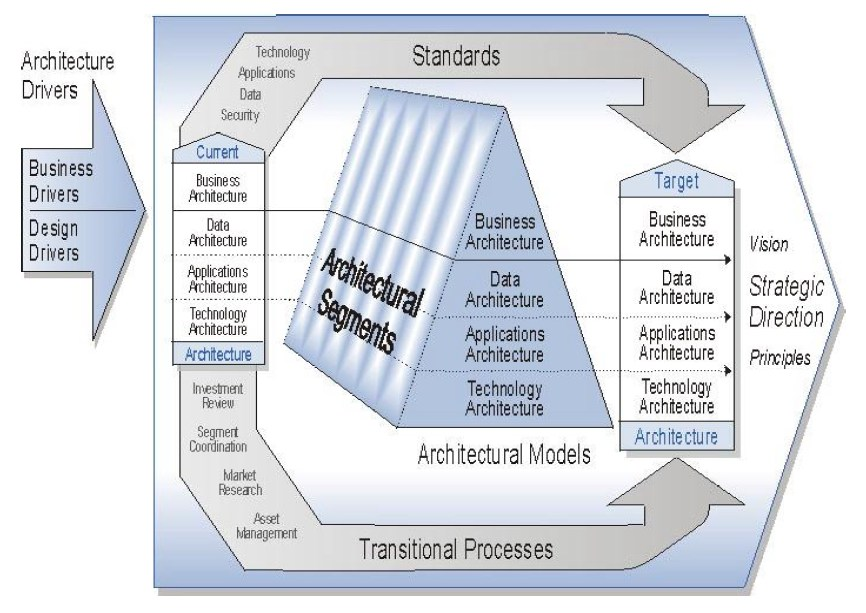
\includegraphics[width=.75\textwidth]{../figures/feaf}
\end{center}

\section{Gartner Enterprise Architecture Method}
Gartner Enterprise Architecture Method dikembangkan oleh perusahaan riset dan konsultasi Gartner. Metode ini membimbing organisasi dalam merancang, mengembangkan, dan menerapkan arsitektur enterprise, menghubungkan strategi bisnis dan TI, serta membantu organisasi mencapai tujuan transformasi digital mereka.

\begin{center}
	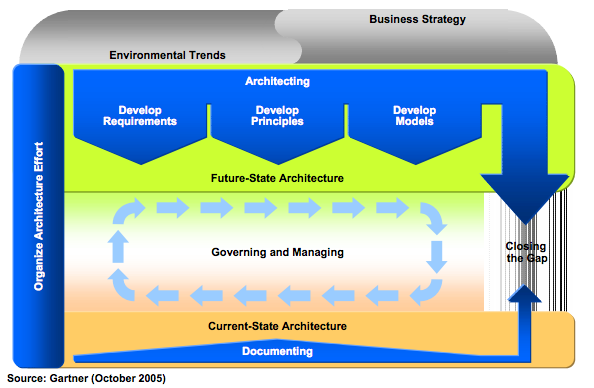
\includegraphics[width=.70\textwidth]{../figures/gartner}
\end{center}

\section{Department of Defense Architecture Framework (DoDAF)}
Department of Defense Architecture Framework (DoDAF) adalah kerangka kerja yang digunakan oleh Departemen Pertahanan AS. Kerangka ini membantu dalam mengorganisir dan memvisualisasikan informasi yang penting untuk proses pengambilan keputusan, menggunakan berbagai model dan panduan untuk mengembangkan arsitektur, dan cocok untuk organisasi dengan kompleksitas dan skala besar.

\begin{center}
	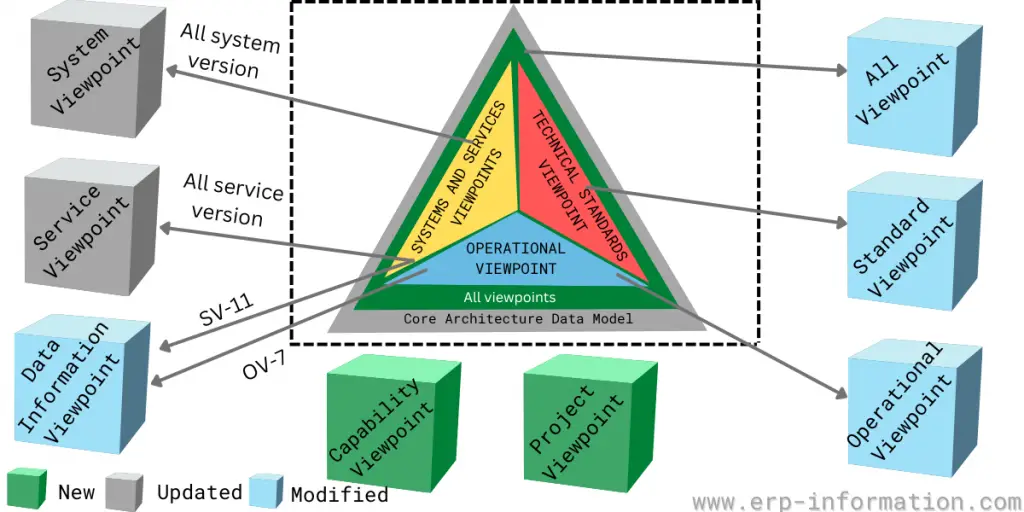
\includegraphics[width=0.68\textwidth]{../figures/dodaf}
\end{center}

\section{Australian Government AGA}
Australian Government AGA adalah kerangka kerja yang digunakan oleh Pemerintah Australia. Kerangka ini membantu dalam perencanaan dan implementasi teknologi informasi di tingkat pemerintah, mendorong kolaborasi antara departemen dan agen pemerintah, serta meningkatkan efisiensi dan transparansi layanan pemerintah.

\begin{center}
	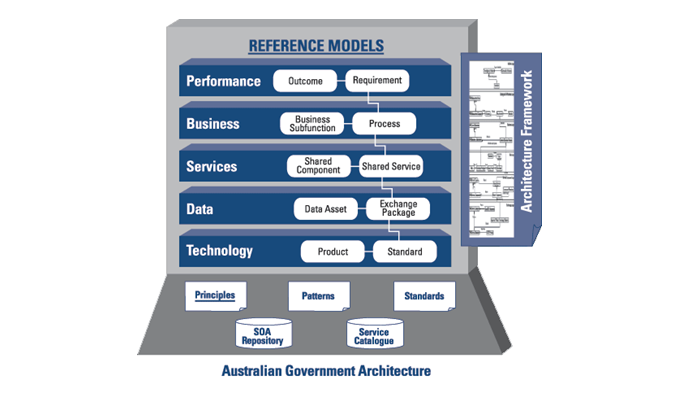
\includegraphics[width=0.9\textwidth]{../figures/aga}
\end{center}

\section{Business Architecture Body of Knowledge (BizBoK)}
Business Architecture Body of Knowledge (BizBoK) adalah panduan yang dikembangkan oleh Business Architecture Guild. Panduan ini menyediakan praktik terbaik dan standar dalam arsitektur bisnis, dapat digunakan oleh arsitek bisnis dan profesional terkait lainnya, serta membantu organisasi dalam merancang dan menerapkan arsitektur bisnis.

\begin{center}
	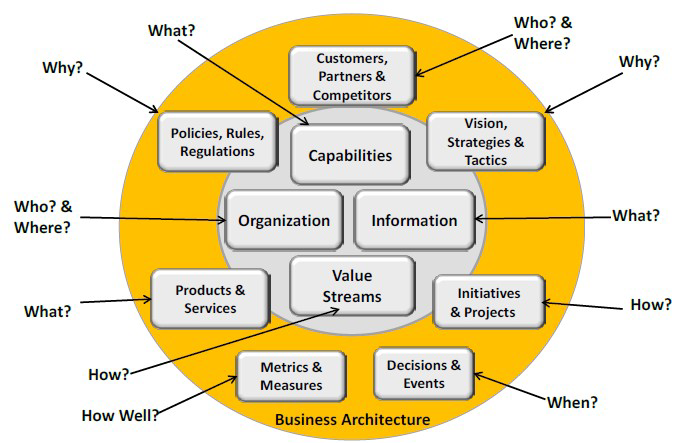
\includegraphics[width=0.7\textwidth]{../figures/bizbok}
\end{center}

\section{ISO Standard for Enterprise Modeling (ISO19439)}
ISO Standard for Enterprise Modeling (ISO19439) adalah standar internasional untuk pemodelan proses bisnis dan organisasi. Standar ini membantu dalam perencanaan, desain, dan perbaikan proses bisnis, dapat digunakan oleh berbagai jenis organisasi, dari bisnis hingga pemerintah, dan dikembangkan oleh Organisasi Internasional untuk Standardisasi (ISO).

\begin{center}
	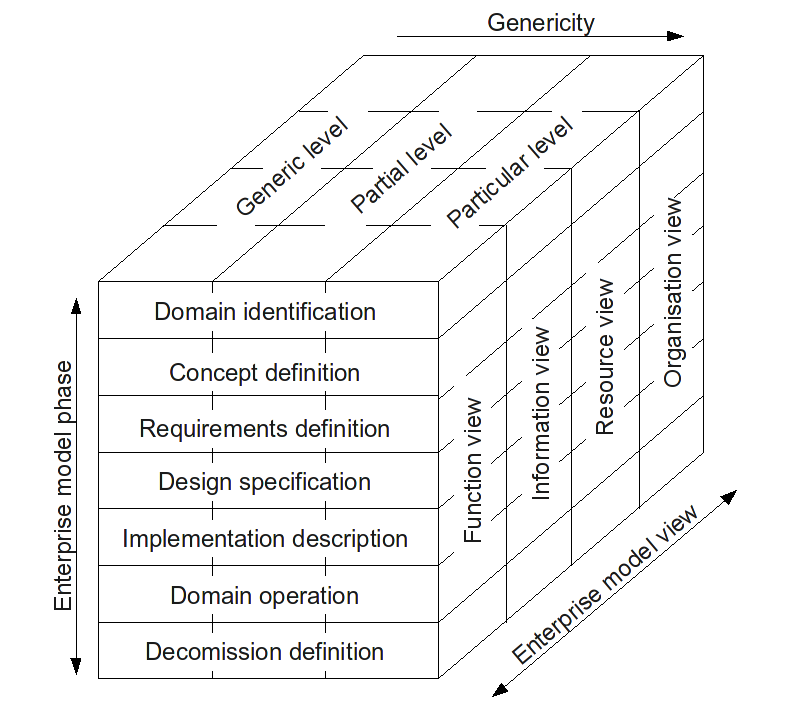
\includegraphics[width=.45\textwidth]{../figures/iso19439}
\end{center}

Terdapat berbagai kerangka dan metodologi arsitektur enterprise yang dapat dipilih sesuai dengan kebutuhan dan konteks spesifik organisasi. Arsitektur enterprise merupakan alat penting untuk perencanaan dan pengelolaan teknologi informasi dalam organisasi.

\section{Kesamaan Antar Kerangka Arsitektur Enterprise}
Meskipun terdapat berbagai kerangka arsitektur enterprise dengan pendekatan dan fokus yang berbeda, beberapa kesamaan mendasar dapat ditemukan di antara mereka:

\begin{itemize}
	\item \textbf{Pendekatan Terstruktur:} Semua kerangka arsitektur enterprise menerapkan pendekatan terstruktur untuk merancang dan mengelola sistem informasi dan TI. Mereka membagi arsitektur menjadi berbagai komponen atau lapisan untuk membantu dalam perencanaan dan implementasi yang lebih baik.
	
	\item \textbf{Fokus pada Keselarasan Strategis:} Kerangka-kerangka ini menekankan pentingnya menyelaraskan teknologi informasi dengan tujuan bisnis organisasi. Mereka berusaha memastikan bahwa keputusan TI mendukung dan memperkuat strategi bisnis keseluruhan.
	
	\item \textbf{Peningkatan Efisiensi dan Efektivitas:} Salah satu tujuan utama dari semua kerangka ini adalah meningkatkan efisiensi dan efektivitas operasional organisasi. Mereka berusaha mengoptimalkan penggunaan sumber daya dan mengurangi kompleksitas dengan memberikan panduan yang jelas dan metodologi yang teruji.
	
	\item \textbf{Manajemen Kompleksitas:} Kerangka-kerangka ini dirancang untuk membantu organisasi dalam mengelola kompleksitas sistem TI dan proses bisnis. Mereka memberikan struktur dan alat untuk memetakan, menganalisis, dan mengelola berbagai aspek arsitektur enterprise.
	
	\item \textbf{Pendekatan Berbasis Model:} Sebagian besar kerangka arsitektur menggunakan model atau representasi visual untuk menggambarkan arsitektur enterprise. Ini membantu dalam memahami hubungan antara berbagai komponen dan bagaimana mereka berinteraksi satu sama lain.
	
	\item \textbf{Fleksibilitas dan Penyesuaian:} Banyak kerangka arsitektur memungkinkan penyesuaian untuk memenuhi kebutuhan spesifik organisasi. Mereka dirancang agar fleksibel dan dapat diterapkan di berbagai konteks dan industri, dari bisnis hingga pemerintahan.
	
	\item \textbf{Penggunaan dalam Perencanaan Strategis:} Kerangka-kerangka ini sering digunakan dalam perencanaan strategis untuk membantu organisasi merumuskan dan mengimplementasikan rencana TI yang selaras dengan tujuan jangka panjang mereka.
\end{itemize}

Dengan kesamaan-kesamaan ini, kerangka arsitektur enterprise memberikan panduan yang kuat untuk organisasi dalam mengelola dan merancang sistem informasi yang efektif dan efisien, meskipun dengan pendekatan dan metode yang berbeda.

\section{Perbedaan Antar Kerangka Arsitektur Enterprise}
Meskipun ada kesamaan di antara berbagai kerangka arsitektur enterprise, perbedaan penting juga ada di antara mereka, yang mencerminkan fokus, metodologi, dan tujuan yang berbeda. Berikut adalah beberapa perbedaan utama:

\begin{itemize}
	\item \textbf{Pendekatan dan Fokus:} Setiap kerangka arsitektur memiliki pendekatan dan fokus yang unik. Misalnya, Framework Zachman menawarkan kerangka kerja berbasis model yang sangat terstruktur untuk manajemen kompleksitas arsitektur, sementara SABSA berfokus pada keamanan dan manajemen risiko dalam konteks arsitektur enterprise.
	
	\item \textbf{Lapisan dan Komponen:} Kerangka arsitektur enterprise dapat memiliki lapisan dan komponen yang berbeda. Sebagai contoh, NIST Enterprise Architecture Model membagi arsitektur TI menjadi lima lapisan yang berbeda, sedangkan Zachman Framework menggunakan enam level berbeda untuk memahami arsitektur dari sudut pandang yang lebih luas.
	
	\item \textbf{Metodologi Pengembangan:} Beberapa kerangka mengikuti metodologi pengembangan tertentu. Misalnya, EAP (Enterprise Architecture Planning) lebih fokus pada perencanaan dan implementasi teknologi baru berdasarkan kebutuhan bisnis, sedangkan Gartner's Enterprise Architecture Method memberikan panduan untuk desain dan implementasi yang berhubungan erat dengan strategi bisnis.
	
	\item \textbf{Penggunaan Model dan Visualisasi:} Setiap kerangka memiliki cara berbeda dalam menggunakan model dan visualisasi. PRISM Architecture Framework, misalnya, menggunakan matriks dan hubungan untuk menggambarkan arsitektur, sementara DoDAF (Department of Defense Architecture Framework) menggunakan berbagai model untuk mendukung proses pengambilan keputusan yang kompleks.
	
	\item \textbf{Aplikasi Sektor dan Konteks:} Beberapa kerangka lebih ditujukan untuk konteks atau sektor tertentu. FEAF (Federal Enterprise Architecture Framework) dirancang khusus untuk pemerintah federal AS, sedangkan Australian Government AGA adalah kerangka kerja yang dirancang untuk meningkatkan efisiensi dan transparansi di tingkat pemerintahan Australia.
	
	\item \textbf{Fleksibilitas dan Penyesuaian:} Derajat fleksibilitas dan penyesuaian juga bervariasi. Beberapa kerangka, seperti Zachman Framework, memiliki struktur yang sangat kaku, terperinci, dan befokus pada artefak, sementara yang lain, seperti SABSA, lebih mudah disesuaikan dengan kebutuhan spesifik keamanan organisasi untuk keperluan bisnis (\textit{business-centric security architectures} dan \textit{risk management frameworks}).
	
	\item \textbf{Standar Internasional:} Kerangka seperti ISO19439 memiliki standar internasional yang mendefinisikan model dan metode untuk perencanaan dan desain proses bisnis, yang mungkin berbeda dengan pendekatan spesifik yang diadopsi oleh kerangka lain.
\end{itemize}

Perbedaan-perbedaan ini mencerminkan variasi dalam kebutuhan organisasi dan konteks di mana kerangka arsitektur diterapkan. Memahami perbedaan ini membantu organisasi memilih kerangka yang paling sesuai dengan tujuan dan tantangan mereka.

\section{Deskripsi Tugas Mata Kuliah Enterprise Architecture}
Untuk membantu kelulusan, mahasiswa diharapkan dapat menghasilkan makalah ilmiah di akhir perkuliahan 1 semester. Model yang dipakailah adalah model flipped classroom di mana mahasiswa akan aktif berpartisipasi dalam perkuliahan. Misalnya, dengan mempresentasikan kemajuan tugas untuk berdiskusi dan mendapatkan umpan balik dari peserta kelas lainnya.

\begin{enumerate}
	\item \textbf{Sesi-01: Introduction to Enterprise Architecture} \\
	\textbf{Tugas}: Identifikasi satu masalah atau peluang di tempat kerja Anda. Anda bisa menggunakan alat-alat analisis seperti SWOT (Strength, Weakness, Opportunity, Threat), Porter's Five Forces, PESTLE (Political, Economic, Social, Technological, Legal, Environmental) ,dsb. Temukan teknologi/inovasi yang dapat meningkatkan kualitas tempat kerja Anda. Identifikasi visi dan misi organisasi tempat Anda bekerja. Wawancarai anggota dewan (\textit{board}), manajer, rekan kerja, atau pihak lain di organisasi tersebut.  Diskusikan ide-ide Anda dengan mereka dan catat umpan balik mereka. Mereka mungkin memberikan ide alternatif atau tambahan. Berdasarkan temuan-temuan ada pada tugas pertemuan sebelumnya, tetapkan \textbf{kemampuan} apa yang perlu ditambahkan ke perusahaan Anda bekerja untuk meningkatkan kualitas bisnisnya. Jadikan itu sebagai studi kasus Anda dan kembangkan arsitektur perusahaan selama semester ini. Ceritakan temuan Anda dalam template makalah.
	
	
	\item \textbf{Sesi-02: Studi Kasus - Remote Working (atau Masalah Lainnya)} \\
	\textbf{Tugas}: 1.) Baca literatur yang membahas TOGAF. 2.) Berdasarkan temuan-temuan ada pada tugas pertemuan sebelumnya, tetapkan kapabilitas/kemampuan apa yang perlu ditambahkan ke perusahaan Anda bekerja untuk meningkatkan kualitas bisnisnya. Selanjutlnya, temukan setidaknya 30 sumber pustaka, termasuk makalah akademik, laporan, white papers, dll.
	
	
	\item \textbf{Sesi-03: TOGAF} \\
	\textbf{Tugas}: Lakukan studi literatur terkait kapabilitas arsitektur Anda. Baca setidaknya 30 sumber, termasuk makalah akademik, laporan, white papers, dll., yang sudah Anda kumpulkan sebelumnya.
	
	\item \textbf{Sesi-04: Preliminary Phase} \\
	\textbf{Tugas}: Definisikan kapabilitas arsitektur Anda, berdasarkan informasi yang dikumpulkan dalam fase Preliminary. Deskripsikan keadaan saat ini (As-Is) dan keadaan target (To-Be) untuk memperjelas kapabilitas tersebut dalam bentuk dokumen \textit{Request for Architectural Work}.
	
	\item \textbf{Sesi-05: Phase A - Architecture Vision} \\
	\textbf{Tugas}: Buatlah visi untuk kapabilitas arsitektur yang Anda pilih, berdasarkan informasi yang dikumpulkan dalam fase Preliminary dan fase ini. Deskripsikan keadaan saat ini (As-Is) dan keadaan target (To-Be) untuk memperjelas visi arsitektur tersebut dalam bentuk kajian kesiapan (Subbab \ref{sec:kesiapan_transformasi}), kajian \textit{stakeholders} (Subbab \ref{sec:stakholders}), perumusan visi arsitektur (Subbab \ref{sec:visi_arsitektur}), kajian skenario bisnis (Subbab \ref{sec:skenario_bisnis}), dan dokumen \textit{Architectural Statement of Work}(Subbab \ref{sec:stament_of_work}).
	
	\item \textbf{Sesi-06: Phase B - Business Architecture} \\
	\textbf{Tugas}: Buat model alur kerja/proses bisnis \textbf{As-Is} yang terpengaruh oleh visi. Juga, buat model alur kerja/proses bisnis \textbf{To-Be} yang diperlukan untuk mewujudkan visi tersebut. Identifikasi kesenjangan dan tindakan yang perlu diambil.
	
	\item \textbf{Sesi-07: Phase C - Data Architecture} \\
	\textbf{Tugas}: Buat model data dan dokumen \textbf{As-Is} yang terpengaruh oleh visi dan proses bisnis/workflows As-Is. Selain itu, buat model data dan dokumen \textbf{To-Be} yang diperlukan untuk mewujudkan visi tersebut dan proses bisnis/workflows To-Be. Identifikasi kesenjangan dan tindakan yang diperlukan.
	
	\item \textbf{Sesi-08: Phase C - Application Architecture} \\
	\textbf{Tugas}: Buat model aplikasi \textbf{As-Is} yang terpengaruh oleh visi, proses bisnis/workflows As-Is, dan model data dan dokumen As-Is. Juga, buat model aplikasi \textbf{To-Be} yang diperlukan untuk mewujudkan visi, termasuk proses bisnis/workflows To-Be dan model data dan dokumen To-Be. Identifikasi kesenjangan dan tindakan yang diperlukan.
	
	\item \textbf{Sesi-09: Phase D - Technology Architecture} \\
	\textbf{Tugas}: Buat model infrastruktur/teknologi \textbf{As-Is} yang terpengaruh oleh visi, proses bisnis/workflows As-Is, model data dan dokumen As-Is, dan model aplikasi As-Is. Juga, buat model infrastruktur/teknologi \textbf{To-Be} yang diperlukan untuk mewujudkan visi, termasuk proses bisnis/workflows To-Be, model data dan dokumen To-Be, dan model aplikasi To-Be. Identifikasi kesenjangan dan tindakan yang diperlukan.
	
	\item \textbf{Sesi-10: Phase E - Opportunities and Solutions} \\
	\textbf{Tugas}: Kelompokkan tindakan dari sesi sebelumnya ke dalam paket kerja dan estimasikan biaya (termasuk jadwal, tenaga kerja, dan sumber daya lainnya) untuk pelaksanaannya. Identifikasi peluang untuk mengoptimalkan pelaksanaan (misalnya, urutan paket kerja, penggabungan tindakan untuk mengurangi biaya).
	
	\item \textbf{Sesi-11: Phase F - Migration Planning} \\
	\textbf{Tugas}: Tuliskan semua pekerjaan Anda dan hasilkan makalah akademik (Shinta 2).
	
	\item \textbf{Sesi-12: Phase G - Implementation Governance} \\
	\textbf{Tugas}: Tuliskan semua pekerjaan Anda dan hasilkan makalah akademik (Shinta 2).
	
	\item \textbf{Sesi-13: Phase H - Architecture Change Management} \\
	\textbf{Tugas}: Tuliskan semua pekerjaan Anda dan hasilkan makalah akademik (Shinta 2). \textbf{Ubah makalah Anda ke dalam bahasa Inggris.}
	
	\item \textbf{Sesi-14: Requirements Management}. Tidak ada tugas
\end{enumerate}


\section{Aktivitas Kelas dan Tugas}
Identifikasi satu masalah atau peluang di tempat kerja Anda. Anda bisa menggunakan alat-alat analisis seperti SWOT (Strength, Weakness, Opportunity, Threat), Porter's Five Forces, PESTLE (Political, Economic, Social, Technological, Legal, Environmental) ,dsb. Temukan teknologi/inovasi yang dapat meningkatkan kualitas tempat kerja Anda.

Identifikasi visi dan misi organisasi tempat Anda bekerja. Wawancarai anggota dewan (\textit{board}), manajer, rekan kerja, atau pihak lain di organisasi tersebut. Diskusikan ide-ide Anda dengan mereka dan catat umpan balik mereka. Mereka mungkin memberikan ide alternatif atau tambahan. Pilih salah satu sebagai studi kasus Anda dan kembangkan arsitektur perusahaan selama semester ini. Ceritakan temuan Anda dalam template makalah. Gunakan template makalah dari makalah terakreditasi \textbf{Shinta 2}.


\section{Contoh Visi dan Misi Organisasi}

\subsection{Visi}
Menjadi institusi pendidikan tinggi yang diakui secara global, mendorong inovasi, integritas, dan inklusivitas, serta membentuk pemimpin yang berkontribusi untuk dunia yang berkelanjutan dan adil.

\subsection{Misi}
\begin{enumerate}
	\item \textbf{Memberikan Pendidikan Berkualitas Tinggi:} Menyediakan pendidikan transformasional yang mempersiapkan mahasiswa untuk unggul di bidang yang dipilih melalui kurikulum mutakhir, pemikiran kritis, dan pengalaman praktis.
	
	\item \textbf{Mendorong Penelitian dan Inovasi:} Menumbuhkan budaya penelitian, kreativitas, dan inovasi untuk menghadapi tantangan masyarakat dan memperkaya ilmu pengetahuan di berbagai disiplin ilmu.
	
	\item \textbf{Membangun Kepemimpinan Etis dan Lingkungan:} Mengembangkan pemimpin dengan rasa etika yang kuat, tanggung jawab sosial, dan kepedulian terhadap lingkungan, mempromosikan praktik berkelanjutan serta komitmen untuk menciptakan perubahan positif di komunitas lokal maupun global.
	
	\item \textbf{Mendorong Inklusivitas dan Keberagaman:} Menciptakan lingkungan belajar yang beragam dan inklusif yang menghargai serta menerima perbedaan, menjamin kesempatan yang setara bagi seluruh anggota komunitas universitas.
	
	\item \textbf{Berkolaborasi dengan Masyarakat:} Membangun kemitraan dengan industri, pemerintah, dan masyarakat sipil untuk menjawab kebutuhan masyarakat dan berkontribusi pada pengembangan bangsa serta dunia.
\end{enumerate}

\section{Contoh Analisis SWOT}

\subsection{Strengths (Kekuatan)}
\begin{itemize}
	\item \textbf{Reputasi Global:} Universitas ini dikenal secara global dengan program akademik berkualitas tinggi dan fokus pada inovasi.
	\item \textbf{Fasilitas Penelitian Unggul:} Dilengkapi dengan laboratorium dan pusat riset yang mendukung inovasi dan penelitian di berbagai disiplin ilmu.
	\item \textbf{Kepemimpinan Etis dan Lingkungan:} Berkomitmen pada pengembangan pemimpin yang tidak hanya etis tetapi juga peduli terhadap keberlanjutan lingkungan.
	\item \textbf{Keragaman dan Inklusivitas:} Universitas ini menawarkan lingkungan yang inklusif dan menghargai keragaman dalam komunitas akademiknya.
\end{itemize}

\subsection{Weaknesses (Kelemahan)}
\begin{itemize}
	\item \textbf{Pendanaan Terbatas untuk Penelitian:} Meskipun memiliki fasilitas unggul, universitas menghadapi keterbatasan dana untuk penelitian di bidang tertentu.
	\item \textbf{Kurangnya Kerjasama Internasional:} Universitas ini masih memiliki peluang untuk meningkatkan kemitraan dengan universitas luar negeri guna memperkuat program pertukaran dan kolaborasi riset.
	\item \textbf{Keterbatasan Program Online:} Pengembangan program pendidikan jarak jauh dan pembelajaran daring masih dalam tahap awal dan belum sepenuhnya optimal.
\end{itemize}

\subsection{Opportunities (Peluang)}
\begin{itemize}
	\item \textbf{Permintaan untuk Pendidikan Berkelanjutan:} Dengan meningkatnya perhatian global terhadap isu lingkungan, ada peluang untuk memperluas program studi yang fokus pada keberlanjutan dan inovasi hijau.
	\item \textbf{Kolaborasi dengan Industri:} Universitas dapat memperluas kemitraan dengan sektor industri untuk meningkatkan relevansi kurikulum dan memperluas peluang magang serta riset terapan.
	\item \textbf{Peningkatan Digitalisasi:} Perkembangan teknologi memungkinkan universitas untuk memperluas jangkauan dengan mengembangkan lebih banyak program pendidikan berbasis daring dan hybrid.
\end{itemize}

\subsection{Threats (Ancaman)}
\begin{itemize}
	\item \textbf{Persaingan Global:} Universitas menghadapi persaingan yang ketat dari institusi-institusi global yang juga menawarkan program berkualitas tinggi dan berfokus pada inovasi.
	\item \textbf{Perubahan Regulasi Pendidikan:} Perubahan kebijakan atau regulasi pemerintah terkait pendidikan tinggi dapat memengaruhi keberlanjutan program dan operasional universitas.
	\item \textbf{Perubahan Tren Pendidikan:} Pergeseran preferensi mahasiswa ke arah pembelajaran daring penuh dapat menurunkan minat terhadap program pendidikan tradisional.
\end{itemize}



\section{Analisis Model Lima Kekuatan Porter}

\subsection{Ancaman Pendatang Baru}
\begin{itemize}
	\item \textbf{Tingkat Persaingan Baru:} Munculnya universitas-universitas baru dengan fokus pada teknologi dan pembelajaran daring dapat meningkatkan persaingan di sektor pendidikan tinggi.
	\item \textbf{Hambatan Masuk yang Tinggi:} Universitas dengan reputasi global dan fasilitas penelitian unggul menghadapi ancaman yang lebih rendah dari pendatang baru, karena membutuhkan investasi besar untuk menyaingi infrastruktur dan reputasi tersebut.
	\item \textbf{Inovasi Teknologi:} Universitas baru yang menawarkan program pendidikan berbasis teknologi mutakhir bisa memberikan alternatif menarik bagi calon mahasiswa.
\end{itemize}

\subsection{Kekuatan Pemasok (Dosen dan Tenaga Ahli)}
\begin{itemize}
	\item \textbf{Ketersediaan Tenaga Ahli:} Universitas membutuhkan tenaga pengajar berkualitas tinggi dengan keahlian khusus. Persaingan dalam menarik dosen-dosen terbaik menjadi tantangan bagi universitas.
	\item \textbf{Ketergantungan pada Pakar:} Ketergantungan yang tinggi pada dosen atau pakar ternama dalam bidang-bidang tertentu dapat menjadi risiko jika mereka pindah ke institusi lain atau berhenti mengajar.
	\item \textbf{Fasilitas Riset dan Inovasi:} Fasilitas penelitian yang unggul memberi universitas daya tarik lebih besar dalam menarik tenaga ahli dan meningkatkan retensi dosen.
\end{itemize}

\subsection{Kekuatan Pembeli (Mahasiswa dan Orang Tua)}
\begin{itemize}
	\item \textbf{Pilihan yang Lebih Luas:} Calon mahasiswa memiliki banyak pilihan untuk universitas lain, termasuk program pembelajaran daring yang mungkin lebih fleksibel dan terjangkau.
	\item \textbf{Tuntutan Mahasiswa:} Mahasiswa semakin menuntut kualitas pendidikan yang lebih baik, fasilitas modern, dan peluang karir yang kuat, sehingga universitas harus terus berinovasi dalam kurikulum dan layanan.
	\item \textbf{Peran Orang Tua:} Orang tua juga memainkan peran penting dalam keputusan memilih universitas, terutama dalam hal biaya pendidikan dan prospek masa depan lulusan.
\end{itemize}

\subsection{Ancaman Produk atau Layanan Pengganti}
\begin{itemize}
	\item \textbf{Pembelajaran Daring:} Program-program pembelajaran daring penuh dari universitas besar atau platform pendidikan seperti Coursera dan edX dapat menjadi ancaman besar bagi universitas yang masih berfokus pada pembelajaran tradisional.
	\item \textbf{Kursus Bersertifikasi:} Sertifikasi profesional yang ditawarkan oleh perusahaan teknologi atau lembaga pelatihan bisa menjadi alternatif bagi mahasiswa yang lebih memilih pembelajaran jangka pendek daripada pendidikan universitas tradisional.
	\item \textbf{Program Magang atau Pelatihan Kerja:} Meningkatnya popularitas program magang langsung atau pelatihan kerja yang diadakan oleh perusahaan juga dapat menjadi alternatif bagi mahasiswa yang menginginkan pengalaman praktis langsung.
\end{itemize}

\subsection{Persaingan Antar Universitas (Rivalitas Kompetitif)}
\begin{itemize}
	\item \textbf{Persaingan Global:} Universitas menghadapi persaingan dari institusi-institusi pendidikan global yang menawarkan program serupa dengan standar internasional, baik secara langsung maupun melalui platform daring.
	\item \textbf{Inovasi Kurikulum:} Universitas lain yang lebih cepat mengadopsi kurikulum inovatif atau pendekatan pembelajaran yang lebih fleksibel dapat menarik lebih banyak mahasiswa.
	\item \textbf{Reputasi dan Jaringan Alumni:} Kekuatan jaringan alumni dan reputasi universitas sangat penting dalam menarik mahasiswa baru dan mempertahankan posisi dalam persaingan.
\end{itemize}

\section{Analisis PESTLE}

\subsection{Faktor Politik}
\begin{itemize}
	\item \textbf{Kebijakan Pendidikan:} Perubahan dalam kebijakan pemerintah terkait pendidikan tinggi dapat mempengaruhi pendanaan, akreditasi, dan regulasi universitas.
	\item \textbf{Stabilitas Politik:} Kondisi politik yang stabil mendukung lingkungan yang kondusif untuk kegiatan akademik dan penelitian.
	\item \textbf{Dukungan Pemerintah:} Program subsidi atau bantuan pemerintah untuk pendidikan tinggi dapat meningkatkan kemampuan universitas dalam menyediakan beasiswa dan fasilitas.
\end{itemize}

\subsection{Faktor Ekonomi}
\begin{itemize}
	\item \textbf{Kondisi Ekonomi:} Kesehatan ekonomi nasional dapat mempengaruhi jumlah dana yang tersedia untuk universitas dan kemampuan mahasiswa untuk membayar biaya kuliah.
	\item \textbf{Pendanaan dan Investasi:} Fluktuasi dalam investasi dan pendanaan dari donor, alumni, dan sponsor industri mempengaruhi kemampuan universitas untuk mengembangkan fasilitas dan program.
	\item \textbf{Biaya Pendidikan:} Kenaikan biaya pendidikan dapat mempengaruhi daya tarik universitas dan jumlah pendaftar, terutama jika biaya kuliah meningkat lebih cepat daripada inflasi.
\end{itemize}

\subsection{Faktor Sosial}
\begin{itemize}
	\item \textbf{Demografi Mahasiswa:} Perubahan dalam demografi, seperti usia, latar belakang etnis, dan lokasi geografis calon mahasiswa, mempengaruhi permintaan untuk program tertentu.
	\item \textbf{Tren Pendidikan:} Preferensi mahasiswa terhadap jenis program dan metode pembelajaran (seperti pembelajaran daring) mempengaruhi strategi kurikulum universitas.
	\item \textbf{Keterlibatan Komunitas:} Keterlibatan universitas dalam kegiatan sosial dan komunitas lokal berkontribusi pada citra dan reputasi institusi.
\end{itemize}

\subsection{Faktor Teknologi}
\begin{itemize}
	\item \textbf{Inovasi Teknologi:} Adopsi teknologi baru dalam pengajaran dan penelitian, seperti alat pembelajaran daring dan perangkat lunak penelitian, meningkatkan daya saing universitas.
	\item \textbf{Keamanan Siber:} Perlunya melindungi data mahasiswa dan penelitian dari ancaman keamanan siber, yang memerlukan investasi dalam infrastruktur TI yang aman.
	\item \textbf{Penelitian dan Pengembangan:} Kemajuan teknologi dapat membuka peluang baru untuk penelitian dan inovasi, serta memperkuat kerjasama dengan industri teknologi.
\end{itemize}

\subsection{Faktor Hukum}
\begin{itemize}
	\item \textbf{Regulasi Pendidikan:} Kepatuhan terhadap regulasi nasional dan internasional mengenai akreditasi, kurikulum, dan hak cipta.
	\item \textbf{Hak Kekayaan Intelektual:} Perlindungan hak cipta dan paten yang dihasilkan dari penelitian universitas.
	\item \textbf{Peraturan Kerja:} Kepatuhan terhadap peraturan ketenagakerjaan dan kebijakan perlindungan hak-hak dosen serta staf.
\end{itemize}

\subsection{Faktor Lingkungan}
\begin{itemize}
	\item \textbf{Kepedulian Lingkungan:} Implementasi kebijakan ramah lingkungan dalam pengelolaan kampus, seperti pengurangan jejak karbon dan penggunaan energi terbarukan.
	\item \textbf{Program Studi Berkelanjutan:} Pengembangan dan penawaran program studi yang fokus pada keberlanjutan dan isu lingkungan.
	\item \textbf{Pengelolaan Sumber Daya:} Praktik pengelolaan sumber daya alam yang efisien untuk mendukung keberlanjutan kampus.
\end{itemize}

\section{Inovasi dan Teknologi IT Terkini untuk Meningkatkan Kualitas Universitas}

\subsection{Pembelajaran Daring dan Hybrid}
\begin{itemize}
	\item \textbf{Platform Pembelajaran Online:} Penggunaan platform seperti Moodle, Blackboard, atau Canvas untuk menyediakan kursus daring, modul pembelajaran, dan interaksi mahasiswa dengan dosen.
	\item \textbf{Kelas Virtual:} Implementasi teknologi kelas virtual seperti Zoom atau Microsoft Teams untuk perkuliahan secara langsung dan sesi diskusi online.
	\item \textbf{Augmented Reality (AR) dan Virtual Reality (VR):} Integrasi AR dan VR untuk memberikan pengalaman belajar yang imersif, seperti simulasi laboratorium atau kunjungan virtual ke lokasi historis.
\end{itemize}

\subsection{Analisis Data dan Kecerdasan Buatan}
\begin{itemize}
	\item \textbf{Sistem Manajemen Pembelajaran Berbasis AI:} Penggunaan kecerdasan buatan untuk menyesuaikan pengalaman belajar dengan kebutuhan individu mahasiswa dan memberikan umpan balik otomatis.
	\item \textbf{Analitik Pembelajaran:} Implementasi alat analitik untuk memantau kemajuan mahasiswa, mengidentifikasi area yang membutuhkan perhatian, dan menyesuaikan kurikulum berdasarkan data kinerja.
	\item \textbf{Chatbot Akademik:} Penggunaan chatbot berbasis AI untuk menjawab pertanyaan mahasiswa tentang administrasi, jadwal, dan materi kuliah secara real-time.
\end{itemize}

\subsection{Keamanan dan Infrastruktur TI}
\begin{itemize}
	\item \textbf{Keamanan Siber:} Implementasi sistem keamanan siber canggih untuk melindungi data mahasiswa dan penelitian dari ancaman cyber, termasuk enkripsi data dan sistem deteksi intrusi.
	\item \textbf{Cloud Computing:} Penggunaan layanan cloud untuk penyimpanan data, kolaborasi, dan skalabilitas, serta untuk meningkatkan fleksibilitas dan efisiensi operasional universitas.
	\item \textbf{Internet of Things (IoT):} Integrasi IoT untuk memantau dan mengelola fasilitas kampus secara lebih efisien, seperti sistem pencahayaan otomatis dan kontrol suhu.
\end{itemize}

\subsection{Pengembangan dan Inovasi Kurikulum}
\begin{itemize}
	\item \textbf{Kursus dan Sertifikasi Online:} Penyediaan kursus online dan sertifikasi yang relevan dengan tren industri terbaru untuk memperluas pengetahuan mahasiswa di luar kurikulum tradisional.
	\item \textbf{Laboratorium Virtual:} Penggunaan laboratorium virtual untuk eksperimen dan praktek yang memungkinkan mahasiswa untuk melakukan penelitian tanpa harus berada di laboratorium fisik.
	\item \textbf{Platform Kolaborasi Penelitian:} Penggunaan platform online untuk kolaborasi penelitian antara mahasiswa, dosen, dan peneliti dari universitas lain atau industri.
\end{itemize}

\subsection{Peningkatan Pengalaman Mahasiswa}
\begin{itemize}
	\item \textbf{Aplikasi Mobile Universitas:} Pengembangan aplikasi mobile untuk memudahkan mahasiswa dalam mengakses informasi kampus, jadwal, materi kuliah, dan layanan administrasi.
	\item \textbf{Sistem Pemantauan Kesehatan Mental:} Implementasi alat dan aplikasi untuk memantau dan mendukung kesehatan mental mahasiswa, seperti platform konseling daring dan aplikasi pelacakan kesejahteraan.
	\item \textbf{Virtual Campus Tours:} Penyediaan tur virtual kampus untuk calon mahasiswa dan orang tua agar dapat menjelajahi fasilitas dan suasana kampus dari jarak jauh.
\end{itemize}

\section{Hasil Wawancara dengan Mahasiswa, Karyawan, dan Dosen}

\subsection{Masalah yang Dihadapi Mahasiswa}
\begin{itemize}
	\item \textbf{Kesulitan Mencari Tempat Parkir:} Mahasiswa mengeluhkan kesulitan dalam menemukan tempat parkir di kampus, terutama selama jam-jam sibuk, yang berdampak pada keterlambatan dan stres.
	\item \textbf{Absensi Manual:} Proses absensi yang masih dilakukan secara manual mengakibatkan keterlambatan dalam pencatatan kehadiran dan memerlukan upaya tambahan untuk verifikasi kehadiran.
	\item \textbf{Dokumen yang Berganda:} Mahasiswa menghadapi masalah dengan dokumen yang harus diisi berulang kali di berbagai tempat, yang menghabiskan waktu dan mengurangi efisiensi.
\end{itemize}

\subsection{Masalah yang Dihadapi Karyawan}
\begin{itemize}
	\item \textbf{Proses Bisnis yang Tidak Jelas:} Karyawan melaporkan bahwa beberapa proses bisnis di universitas belum terdokumentasi dengan baik atau tidak jelas, mengakibatkan kebingungan dan ketidakpastian dalam pelaksanaan tugas.
	\item \textbf{Tanggung Jawab Tidak Jelas:} Ada ketidakjelasan mengenai pembagian tanggung jawab dan wewenang di beberapa departemen, yang menyebabkan konflik dan keterlambatan dalam penyelesaian pekerjaan.
	\item \textbf{Dokumentasi Internal yang Berganda:} Pengelolaan dokumen internal yang tidak terintegrasi menyebabkan adanya salinan dokumen yang berulang dan berpotensi memicu kesalahan atau kehilangan informasi.
\end{itemize}

\subsection{Masalah yang Dihadapi Dosen}
\begin{itemize}
	\item \textbf{Keterlambatan Administrasi:} Dosen mengalami keterlambatan dalam proses administrasi, seperti pendaftaran mata kuliah dan pengolahan nilai, yang mengganggu efisiensi dan jadwal pengajaran.
	\item \textbf{Kurangnya Alat Bantu Pengajaran:} Dosen melaporkan kurangnya alat bantu pengajaran dan teknologi yang memadai untuk mendukung proses pembelajaran dan penelitian.
	\item \textbf{Komunikasi yang Tidak Efisien:} Masalah dalam komunikasi antara dosen dan administrasi atau antara dosen dengan mahasiswa menyebabkan kebingungan dan keterlambatan dalam menyelesaikan tugas atau masalah akademik.
\end{itemize}



